\section{Introduction}

\subsection{Context \& background}
\frame {
  \frametitle{Real-time systems}
  \begin{definition}
    A \alert{real-time} system is one in which the validity of a
    computation is dependant not only on the result of said
    computation, but also on the time it is available
  \end{definition}
  \pause
  \begin{center}
    $
\includegraphics[scale=0.8]{../figs/hard_vs_soft}$
  \end{center}
}

\frame {
  \frametitle{Code generation}
  \begin{itemize}
    \item When code is not written by hand, it is code generation
    \item Can't come out of thin air
    \pause
    \item Comes from a \alert{model}
  \end{itemize}
  \pause
  \begin{definition}
    A \alert{model} is an abstraction of a system
  \end{definition}
  \textbf{System:} Cannonball fired from a cannon\\
  \textbf{Model:} Equation of projectile with bound variables\\
  \textcolor{gray}{\textbf{Meta-model:} Equation of projectile with
    unbound variables}\\
  \textcolor{LightGray}{\textbf{Meta-meta-model:} Calculus}
}

\frame {
  \frametitle{Software models and MDE (Model Driven Engineering)}
  \begin{itemize}
    \item Software is also approximated by models
    \item Old idea, now evolving into something quite useful
      \pause
    \item Flowcharts$\to$JSD$\to$OMT \& OOSE$\to$UML
    \item Models becoming part of SDLC (S/W Dev. Lifecycle)
    \item Mainly the design and coding part is affected by MDE
    \item To a lesser extent also testing and deployment
    \item Lots of modeling methods, most prevalent example: UML
  \end{itemize}
}

\frame {
  \frametitle{S/W Development Lifecycle: The MDE approach}
  \begin{center}
    $\includegraphics[scale=0.7]{../figs/mde_presentation_generic}$
  \end{center}
}

\frame {
  \frametitle{Verification}
  \begin{itemize}
    \item Use a mathematically precise way to describe a system
    \item Run the mathematical description of the system
    \item Explore \emph{all} possible states the system can go into
    \item Determine whether/which properties hold in which states
    \item Reason based on those properties
  \end{itemize}
}

\frame {
  \frametitle{Context of work}
  But what did \emph{you} do?
  \pause
  \begin{itemize}
    \item Worked in ASSERT European Project
    \item Large consortium, to do what?
      \pause
    \item To use formal methods and MDE to make more robust real-time
      software
  \end{itemize}
  \pause
  OK, but what \emph{part} did you do?
  \pause
  \begin{itemize}
    \item Use a new architecture description language to generate code
      for hard real-time systems
    \item Perform some verifications on the code generated
  \end{itemize}
}

\frame {
  \frametitle{What modeling language? What executive?}
  Code generation from the AADL...
  \pause
  \begin{itemize}
    \item Architecture Analysis \& Design Language (V1, 2004)
    \item Descendant of MetaH
    \item Tailored to the real-time and safety-critical domain
    \item Developed by SAE
  \end{itemize}
  \pause
  ... to the Ada Ravenscar Profile
  \begin{itemize}
    \item Ada Ravenscar, a profile (subset) of Ada
    \item Intended for use in high-integrity hard real-time systems
    \item Provides certain safety guarantees and analysis possibilities
  \end{itemize}
}

\frame {
  \frametitle{A picture is worth...}
  $\includegraphics[scale=0.7]{../figs/mde_presentation}$
}

\subsection{Survey}

\frame {
  \frametitle{Aren't there others?}
  Of course there are, I even showed some
  \pause
  \begin{itemize}
    \item Dozens of modeling methodologies
    \item Some mainstream, some niche
    \item Some famous, some unknown
      \pause
    \item Ones pertinent to the domain
      \begin{itemize}
        \item UML
        \item UML profiles
        \item SCADE, Simulink
      \end{itemize}
  \end{itemize}
}

\frame {
  \frametitle{UML}
  \begin{itemize}
    \item General purpose modeling language
    \item Initially a graphical representation for OO concepts
    \item Now has concepts like functional modeling \& decomposition
    \item Tools like Rhapsody furnish a modicum of RT support
  \end{itemize}
  \pause
  \textbf{Advantages}
  \begin{itemize}
    \item Inclusionist approach, accomodates everyone, allows
      extensions (which is why it's a good PIM)
    \item Some support for real-time from Rhapsody and similar tools
  \end{itemize}
  \pause
  \textbf{Disadvantages}
  \begin{itemize}
    \item Complex compared to AADL, ambiguous semantics
    \item Strongly tied to OO concepts
    \item Absence of runtime constructs, needs \alert{semantic
      overloading}
  \end{itemize}
}

\frame {
  \frametitle{HRT-UML}
  \begin{itemize}
    \item{A profile of UML for hard real-time systems}
    \item{Closely tied to the Ravenscar Profile for HI systems}
    \item{\emph{Stereotypes} like {\footnotesize $\ll PERIODIC\gg$, $\ll
        SPORADIC\gg$}}
    \item{{\footnotesize PERIOD, DEADLINE, PRIORITY} become meta-attributes}
  \end{itemize}
  \pause
  \textbf{Advantages}
  \begin{itemize}
    \item Explicit modeling of HRT concepts
    \item Ravenscar Profile$\implies$safety
    \item Allows \emph{a priori} schedulability analysis
  \end{itemize}
  \pause
  \textbf{Disadvantages}
  \begin{itemize}
    \item Enforces a low level of abstraction
    \item Engages in more \alert{semantic overload}
  \end{itemize}
}

\frame {
  \frametitle{Lustre \& SCADE Suite}
  \begin{itemize}
    \item{Synchronous data flow programming language}
    \item{Primary use in reactive and control systems}
    \item{System is set of \alert{nodes}, operate in lockstep}
    \item{SCADE Suite, an industrial version of the language}
  \end{itemize}
  \pause
  \textbf{Advantages}
  \begin{itemize}
    \item Mathematically sound, allows model checking
    \item Good abstraction level of control system concepts
    \item Robust, deterministic execution
  \end{itemize}
  \pause
  \textbf{Disadvantages}
  \begin{itemize}
    \item Synchronous execution model, cyclic executive
    \item No aperiodic threads, all periods harmonic
    \item Not suited to general real-time systems
  \end{itemize}
}

%%%%%%%%%%%%%%%%%%%%%%%%%%%%%%%%%%%%%%%%%%%%%%%%%%%%%
\begin{comment}

\frame {
  \frametitle{Lustre \& SCADE Suite}
  %\begin{minipage}{0.45\linewidth}
    \textbf{Advantages}
    \begin{itemize}
      \item{Mathematically sound method}
      \item{Provides robust \& deterministic execution}
      \item{Provides direct abstraction of control system concepts at
        software level}
      \item{Model checking possible because of internal automata-based
        representation}
    \end{itemize}
  %\end{minipage}
  %\hspace{2mm}
  %\begin{minipage}{0.45\linewidth}
    \pause
    \textbf{Disadvantages}
    \begin{itemize}
      \item{Is a synchronous, thus implemented via a cyclic executive,
        which precludes true aperiodic tasks}
      \item{Potential wastage of processor cycles}
      \item{Implies zero execution time semantics}
      \item{Not well-suited to real-time systems other than control
        systems}
    \end{itemize}
  %\end{minipage}
}

\frame {
  \frametitle{HRT-UML (contd.)}
  %\begin{minipage}{0.45\linewidth}
    \textbf{Advantages}
    \begin{itemize}
      \item{Folds the design into UML}
      \item{Explicit modeling of hard real-time constructs}
      \item{\emph{Might} allow inclusion of functional modeling via
        statecharts}
      \item{Offline, \emph{a priori} schedulability analysis}
    \end{itemize}
  %\end{minipage}
  \hspace{2mm}
  %\begin{minipage}{0.45\linewidth}
    \pause
    \textbf{Disadvantages}
    \begin{itemize}
      \item{Folds the design into UML}
      \item{More semantic overload than vanilla UML}
      \item{Enforces a low level of abstraction for concepts. Is a
        graphical representation of the software concepts}
    \end{itemize}
  %\end{minipage}
}

\frame {
  \frametitle{Requirements}
  \begin{minipage}{0.45\linewidth}
    \begin{itemize}
      \item<1->{\alert{Functional}}
      \item<2->{\alert{Non-functional}}
    \end{itemize}
  \end{minipage}
  \hspace{2mm}
  \begin{minipage}{0.45\linewidth}
    \begin{itemize}
      \item<1->{$y = f(x)$}
      \item<2->{Timing, memory, GUI$\ldots$}
    \end{itemize}
  \end{minipage}
  \vspace{3mm}
  \pause
  \pause
  \begin{itemize}
    \item{Traditional systems place premium on functional
      requirements}
    \item{Breach of functional requirements breaks \emph{mission}}
    \item{A word processor that does not save a file}
      \pause
      \vspace{3mm}
    \item{Breach of non-functional requirements \emph{may} be
      inconvenience}
    \item{\emph{May} be more than a mere inconvenience}
    \item{A word processor that saves a file in 30 secs}
  \end{itemize}

  \pause
  \begin{definition}
    The \alert{validity} of a computational result is the inverse of
    the amount of deviation it causes from the system's set of
    requirements
  \end{definition}
}

\subsection{Real-time systems}
\begin{frame}
  \frametitle{Real-time systems}
  \begin{minipage}{0.4\linewidth}
    \begin{itemize}
      \item<1->{Traditional}
      \item<2->{Real-time}
    \end{itemize}
  \end{minipage}
  \begin{minipage}{0.56\linewidth}
    \begin{itemize}
      \item<1->{$Result\ validity = f (value)$}
      \item<2->{$Result\ validity = f (value, time)$}
    \end{itemize}
  \end{minipage}
  \vspace{3mm}
  \pause
  \pause
  \begin{definition}
    A \alert{real-time} system is one in which the validity of a
    computation is dependant not only on the result of said
    computation, but also on the time it is available
  \end{definition}

  \pause
  \begin{itemize}
    \item{Industrial process control \& monitoring}
    \item{Vehicular and platform control}
    \item{Vehicular status monitoring and sensors (GPS etc.)}
    \item{Multimedia systems}
  \end{itemize}
\end{frame}

\frame {
  \frametitle{Classes of real-time systems}
  \begin{center}
    \uncover<1->{$
\includegraphics[scale=0.8]{../figs/hard_vs_soft}$}
    \uncover<2->{$\includegraphics[scale=0.6]{../figs/rt_apps_overview}$}
  \end{center}
}

\subsection{High-integrity \& safety-critical software}
\frame {
  \frametitle{HI and SC software}
  \begin{description}
    \item[High-integrity:]{Software on which are leveraged stringent
      requirements of correctness, robustness \& availability}
    \item[Safety-critical:]{Software on which a fault \alert{may}
      endanger human life}
  \end{description}
  \begin{itemize}
    \item<2->{Vehicular management (cruise control, autopilot)}
    \item<2->{Assembly lines}
    \item<3->{Medical devices (radiation machines, X-rays, MRIs)}
    \item<3->{Mission management systems (GNC, GPS, $\ldots$)}
    \item<4->{Control systems (fly-by-wire, drive-by-wire, anti-lock
      braking)}
  \end{itemize}
  \pause
  \begin{block}{Why?}
    \begin{itemize}
      \item<2->{Reduction of labor via automation}
      \item<3->{Introduction of functionality}
      \item<4->{Maintaining platform stability}
    \end{itemize}
  \end{block}
}

\frame {
  \frametitle{Certification}
  \begin{itemize}
    \item{Most safety-critical software is \alert{certified}}
    \item{Certification entails an audit by a---usually
      government---agency}
    \item{Certification is necessary for deployment of software}
    \item{Certification may be achieved via
      \begin{itemize}
        \item{Manual inspection of code}
        \item{Formal verification}
        \item{Proofs}
      \end{itemize}
    }
      \pause
    \item{ANS7432: Application Criteria for Safety Systems of Nuclear
      Power Generating Stations}
    \item{DO-178B: Software Considerations in Airborne Systems and
      Equipment Certification}
  \end{itemize}
}

\frame{
  \frametitle{DO-178B \& the SDLC}
  \begin{itemize}
    \item{DO-178B is the certification standard for aerospace
      software}
    \item{Is \alert{not} an SDLC}
    \item{Leverages requirements on each phase of the SDLC chosen}
    \item{Most requirements are documentation, some testing
      requirements as well}
  \end{itemize}
  \pause
  {\footnotesize
  \begin{table}
    \centering
    \begin{tabular}{|l|l|l|}
      \hline
      \textbf{Software level}&\textbf{Failure condition}&\textbf{Outcome}\\
      \hline
      Level A & Catastrophic & Death or injury\\
      Level B & Hazardous/Severe-major & Injury\\
      Level C & Major & Unsafe workload\\
      Level D & Minor & Increased workload\\
      Level E & No effect & None\\
      \hline
    \end{tabular}
    \caption{DO-178B Safety Criticality Levels}
  \end{table}
  }
}

\subsection{Model driven engineering}

\frame {
  \frametitle{Make models, not code}
  Model driven engineering is an approach to development where
  \begin{quote}
    models are the primary artifacts of development and developers
    rely on computer-based technologies to transform models to running
    systems
  \end{quote}
  \pause
  \begin{itemize}
    \item{A model is an approximation or an abstraction of a system}
    \item{It abstracts away complexity, thus is easier to construct}
      \pause
    \item{Models can be used for one of three purposes
      \pause
      \begin{enumerate}
        \item{Documentation}
          \pause
        \item{Analysis}
          \pause
        \item{Code generation}
      \end{enumerate}
    }
  \end{itemize}
}

\frame {
  \frametitle{MDE in SDLC}
  \begin{itemize}
    \item{System requirements are captured}
    \item{Functional specifications are given}
    \item{\alert{System design is constructed}}
    \item{\alert{Code is written---or generated---corresponding to
        design}}
    \item{Modules are tested}
    \item{Modules are integrated}
    \item{System is deployed}
  \end{itemize}
}
\frame {
  \frametitle{MDE in the SDLC}
  \begin{center}
    $\includegraphics[scale=0.78]{../figs/mde_chain}$
  \end{center}
}

\subsection{Motivation and context of contribution}

\frame {
  \frametitle{Handling real-time system complexity}
  \begin{itemize}
    \item{Complexity of real-time systems increasing
      \begin{itemize}
        \item{More complex systems being constructed}
        \item{More functionality being demanded, the \emph{``give me
            more''} effect}
        \item{Vicious circle (more compute power$\to$more
          functionality$\to$more compute power)}
        \item{Faster times-to-market}
      \end{itemize}
    }
    \item{Becoming unfeasible to write code by hand}
    \item{Manual coding increases chances of errors}
    \item{Thus MDE approach even more pertinent for HI, RT systems}
  \end{itemize}
}

\frame {
  \frametitle{Motivation for work}
  \begin{itemize}
    \item{Various MDE approaches exist, some general, some tailored
      for real-time systems}
    \item{\textbf{UML:} general purpose. Tool-dependant support for
      real-time systems, generates functional and framework code}
    \item{\textbf{ADLs:} Architecture Description Languages such as
      Rapide, Write, etc. which provide a higher-level view of
      systems}
      \item{\textbf{UML Profiles:} specializations of UML such as
        MARTE and HRT-UML specifically tailored for real-time systems}
      \item{\textbf{Synchronous:} model-driven synchronous approaches
        such as Lustre and MATLAB \simu that generate control system
        code from high-level system models}
  \end{itemize}
}
\end{comment}
